\documentclass[twoside]{book}

% Packages required by doxygen
\usepackage{fixltx2e}
\usepackage{calc}
\usepackage{doxygen}
\usepackage[export]{adjustbox} % also loads graphicx
\usepackage{graphicx}
\usepackage[utf8]{inputenc}
\usepackage{makeidx}
\usepackage{multicol}
\usepackage{multirow}
\PassOptionsToPackage{warn}{textcomp}
\usepackage{textcomp}
\usepackage[nointegrals]{wasysym}
\usepackage[table]{xcolor}

% Font selection
\usepackage[T1]{fontenc}
\usepackage[scaled=.90]{helvet}
\usepackage{courier}
\usepackage{amssymb}
\usepackage{sectsty}
\renewcommand{\familydefault}{\sfdefault}
\allsectionsfont{%
  \fontseries{bc}\selectfont%
  \color{darkgray}%
}
\renewcommand{\DoxyLabelFont}{%
  \fontseries{bc}\selectfont%
  \color{darkgray}%
}
\newcommand{\+}{\discretionary{\mbox{\scriptsize$\hookleftarrow$}}{}{}}

% Page & text layout
\usepackage{geometry}
\geometry{%
  a4paper,%
  top=2.5cm,%
  bottom=2.5cm,%
  left=2.5cm,%
  right=2.5cm%
}
\tolerance=750
\hfuzz=15pt
\hbadness=750
\setlength{\emergencystretch}{15pt}
\setlength{\parindent}{0cm}
\setlength{\parskip}{0.2cm}
\makeatletter
\renewcommand{\paragraph}{%
  \@startsection{paragraph}{4}{0ex}{-1.0ex}{1.0ex}{%
    \normalfont\normalsize\bfseries\SS@parafont%
  }%
}
\renewcommand{\subparagraph}{%
  \@startsection{subparagraph}{5}{0ex}{-1.0ex}{1.0ex}{%
    \normalfont\normalsize\bfseries\SS@subparafont%
  }%
}
\makeatother

% Headers & footers
\usepackage{fancyhdr}
\pagestyle{fancyplain}
\fancyhead[LE]{\fancyplain{}{\bfseries\thepage}}
\fancyhead[CE]{\fancyplain{}{}}
\fancyhead[RE]{\fancyplain{}{\bfseries\leftmark}}
\fancyhead[LO]{\fancyplain{}{\bfseries\rightmark}}
\fancyhead[CO]{\fancyplain{}{}}
\fancyhead[RO]{\fancyplain{}{\bfseries\thepage}}
\fancyfoot[LE]{\fancyplain{}{}}
\fancyfoot[CE]{\fancyplain{}{}}
\fancyfoot[RE]{\fancyplain{}{\bfseries\scriptsize Generated on Tue Oct 20 2015 19\+:55\+:48 for Potts\+Sim by Doxygen }}
\fancyfoot[LO]{\fancyplain{}{\bfseries\scriptsize Generated on Tue Oct 20 2015 19\+:55\+:48 for Potts\+Sim by Doxygen }}
\fancyfoot[CO]{\fancyplain{}{}}
\fancyfoot[RO]{\fancyplain{}{}}
\renewcommand{\footrulewidth}{0.4pt}
\renewcommand{\chaptermark}[1]{%
  \markboth{#1}{}%
}
\renewcommand{\sectionmark}[1]{%
  \markright{\thesection\ #1}%
}

% Indices & bibliography
\usepackage{natbib}
\usepackage[titles]{tocloft}
\setcounter{tocdepth}{3}
\setcounter{secnumdepth}{5}
\makeindex

% Hyperlinks (required, but should be loaded last)
\usepackage{ifpdf}
\ifpdf
  \usepackage[pdftex,pagebackref=true]{hyperref}
\else
  \usepackage[ps2pdf,pagebackref=true]{hyperref}
\fi
\hypersetup{%
  colorlinks=true,%
  linkcolor=blue,%
  citecolor=blue,%
  unicode%
}

% Custom commands
\newcommand{\clearemptydoublepage}{%
  \newpage{\pagestyle{empty}\cleardoublepage}%
}


%===== C O N T E N T S =====

\begin{document}

% Titlepage & ToC
\hypersetup{pageanchor=false,
             bookmarks=true,
             bookmarksnumbered=true,
             pdfencoding=unicode
            }
\pagenumbering{roman}
\begin{titlepage}
\vspace*{7cm}
\begin{center}%
{\Large Potts\+Sim \\[1ex]\large 1.\+0 }\\
\vspace*{1cm}
{\large Generated by Doxygen 1.8.10}\\
\vspace*{0.5cm}
{\small Tue Oct 20 2015 19:55:48}\\
\end{center}
\end{titlepage}
\clearemptydoublepage
\tableofcontents
\clearemptydoublepage
\pagenumbering{arabic}
\hypersetup{pageanchor=true}

%--- Begin generated contents ---
\chapter{readme}
\label{md__home_deathquasar__projects__m_h_p_c__thesis__code__potts_code_bench_readme}
\hypertarget{md__home_deathquasar__projects__m_h_p_c__thesis__code__potts_code_bench_readme}{}
\#\+Benchmarks From this folder is possible to run multiple benchmarks. Every type of benchmark is stored inside the proper folder. Each benchmark has a run\+\_\+bench.\+sh which defines the benchmark. Here is the list of the supported benchmarks.

\subsection*{standard}

With a fixed configuration print the initialization and dynamics times (for all the implemented strategies).

\subsection*{parameters\+\_\+sweeping}

Does a simple parameters sweeping of parameters that can be changed inside the run\+\_\+bench.\+sh script.

\#\+Reports

Main results will be presented inside this folder. 
\chapter{readme}
\label{md__home_deathquasar__projects__m_h_p_c__thesis__code__potts_code_bench_reports_ulisseno_exit_bench_readme}
\hypertarget{md__home_deathquasar__projects__m_h_p_c__thesis__code__potts_code_bench_reports_ulisseno_exit_bench_readme}{}
Test run on ulisse, with 1500 units different connecitivty but no exit condition 
\chapter{readme}
\label{md__home_deathquasar__projects__m_h_p_c__thesis__code__potts_code_bench_standard_readme}
\hypertarget{md__home_deathquasar__projects__m_h_p_c__thesis__code__potts_code_bench_standard_readme}{}
\#\+Standard Bench This benchmark is a general benchmark that runs and compare the new and the old code in one configuration and print on standard output the timings. 
\chapter{Potts simulation model}
\label{md__home_deathquasar__projects__m_h_p_c__thesis__code__potts_code_readme}
\hypertarget{md__home_deathquasar__projects__m_h_p_c__thesis__code__potts_code_readme}{}
\subsection*{Running the stable code}

To compile the code in terminal use {\itshape make} or instead to compile and run, write {\itshape make run}. Do not break the directory tree to keep makefiles and scripts fully working.

\subsection*{Folder structure}


\begin{DoxyItemize}
\item {\itshape bench} \+: Keeps some useful benchmarks, more info in the readme inside the folder.
\item {\itshape build} \+: Default directory where the binaries are going to be generated
\item {\itshape include} \+: Default directory that keeps the \char`\"{}frontend\char`\"{} includes
\item {\itshape src} \+: Default directory that keeps the source files.
\item {\itshape lib} \+: Default directory that keeps all the .cpp and .h used in a generic source file.
\item {\itshape tests} \+: Directory in which is possible to run some regression tests 
\end{DoxyItemize}
\chapter{readme}
\label{md__home_deathquasar__projects__m_h_p_c__thesis__code__potts_code_tests_readme}
\hypertarget{md__home_deathquasar__projects__m_h_p_c__thesis__code__potts_code_tests_readme}{}
\#\+Test Inside this folder you can run {\itshape make test} so that some tests will be performed in order to check that the numbers are the same as in the old code. 
\chapter{Hierarchical Index}
\section{Class Hierarchy}
This inheritance list is sorted roughly, but not completely, alphabetically\+:\begin{DoxyCompactList}
\item \contentsline{section}{parameters}{\pageref{structparameters}}{}
\item \contentsline{section}{Pattern\+Gen}{\pageref{classPatternGen}}{}
\item \contentsline{section}{P\+Net}{\pageref{classPNet}}{}
\begin{DoxyCompactList}
\item \contentsline{section}{H\+C\+\_\+\+P\+Net}{\pageref{classHC__PNet}}{}
\item \contentsline{section}{L\+C\+\_\+\+P\+Net}{\pageref{classLC__PNet}}{}
\begin{DoxyCompactList}
\item \contentsline{section}{V\+L\+C\+\_\+\+P\+Net}{\pageref{classVLC__PNet}}{}
\end{DoxyCompactList}
\end{DoxyCompactList}
\item \contentsline{section}{P\+PS}{\pageref{classPPS}}{}
\item \contentsline{section}{Random\+Sequence}{\pageref{classRandomSequence}}{}
\end{DoxyCompactList}

\chapter{Class Index}
\section{Class List}
Here are the classes, structs, unions and interfaces with brief descriptions\+:\begin{DoxyCompactList}
\item\contentsline{section}{\hyperlink{class_h_c___p_net}{H\+C\+\_\+\+P\+Net} }{\pageref{class_h_c___p_net}}{}
\item\contentsline{section}{\hyperlink{class_l_c___p_net}{L\+C\+\_\+\+P\+Net} }{\pageref{class_l_c___p_net}}{}
\item\contentsline{section}{\hyperlink{structparameters}{parameters} }{\pageref{structparameters}}{}
\item\contentsline{section}{\hyperlink{class_pattern_gen}{Pattern\+Gen} }{\pageref{class_pattern_gen}}{}
\item\contentsline{section}{\hyperlink{class_p_net}{P\+Net} }{\pageref{class_p_net}}{}
\item\contentsline{section}{\hyperlink{class_p_p_s}{P\+P\+S} }{\pageref{class_p_p_s}}{}
\item\contentsline{section}{\hyperlink{class_random_sequence}{Random\+Sequence} }{\pageref{class_random_sequence}}{}
\item\contentsline{section}{\hyperlink{class_v_l_c___p_net}{V\+L\+C\+\_\+\+P\+Net} }{\pageref{class_v_l_c___p_net}}{}
\end{DoxyCompactList}

\chapter{Class Documentation}
\hypertarget{class_h_c___p_net}{}\section{H\+C\+\_\+\+P\+Net Class Reference}
\label{class_h_c___p_net}\index{H\+C\+\_\+\+P\+Net@{H\+C\+\_\+\+P\+Net}}
Inheritance diagram for H\+C\+\_\+\+P\+Net\+:\begin{figure}[H]
\begin{center}
\leavevmode
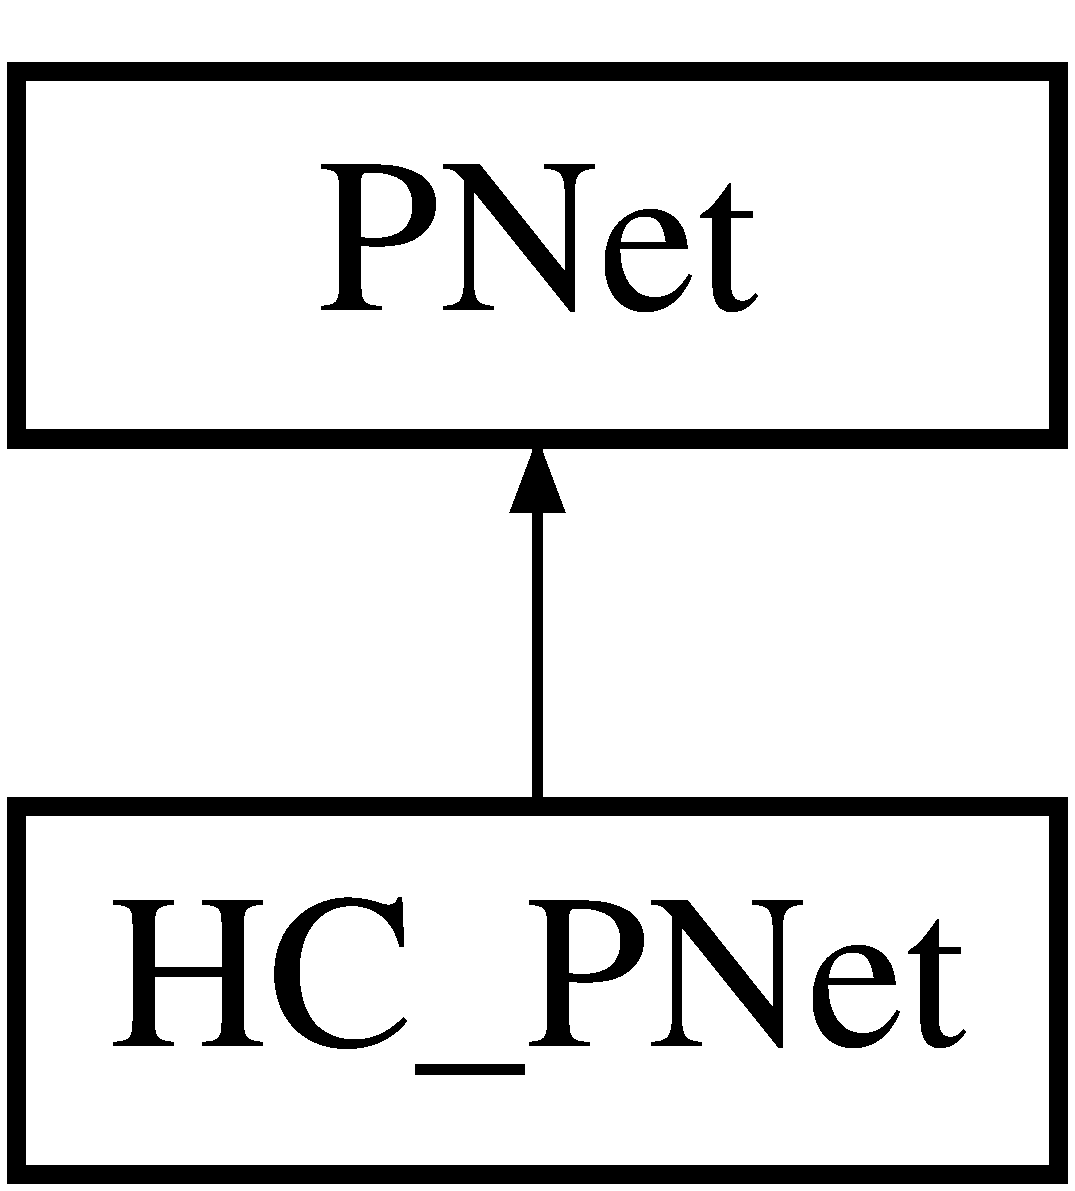
\includegraphics[height=2.000000cm]{class_h_c___p_net}
\end{center}
\end{figure}
\subsection*{Public Member Functions}
\begin{DoxyCompactItemize}
\item 
\hypertarget{class_h_c___p_net_a5c7aca1e9fa59ca5aee29894de0b970f}{}{\bfseries H\+C\+\_\+\+P\+Net} (const int \&N, const int \&C, const int \&S)\label{class_h_c___p_net_a5c7aca1e9fa59ca5aee29894de0b970f}

\item 
\hypertarget{class_h_c___p_net_a91cd9aaa6acbf80f6dcca26ba1e5cd4f}{}void {\bfseries import\+\_\+connections} (const std\+::string \&filename)\label{class_h_c___p_net_a91cd9aaa6acbf80f6dcca26ba1e5cd4f}

\item 
\hypertarget{class_h_c___p_net_a49ff9fe01c408c0c028d736135dd4ef3}{}void {\bfseries print\+\_\+cm} ()\label{class_h_c___p_net_a49ff9fe01c408c0c028d736135dd4ef3}

\item 
\hypertarget{class_h_c___p_net_a0f1e9277e2f5320ff638c9d6adf7c1db}{}void {\bfseries save\+\_\+states\+\_\+to\+\_\+file} (const std\+::string \&filename)\label{class_h_c___p_net_a0f1e9277e2f5320ff638c9d6adf7c1db}

\item 
\hypertarget{class_h_c___p_net_a7d72eed734dc1a8c42f760db4ce19f0a}{}void {\bfseries save\+\_\+connections\+\_\+to\+\_\+file} (const std\+::string \&filename)\label{class_h_c___p_net_a7d72eed734dc1a8c42f760db4ce19f0a}

\item 
\hypertarget{class_h_c___p_net_aaf22bc06a174cbe262a0ddbceb8cb079}{}void {\bfseries save\+\_\+\+J\+\_\+to\+\_\+file} (const std\+::string \&filename)\label{class_h_c___p_net_aaf22bc06a174cbe262a0ddbceb8cb079}

\item 
\hypertarget{class_h_c___p_net_a404e5bb38475c42180d615e2dda8418d}{}void {\bfseries connect\+\_\+units} (std\+::default\+\_\+random\+\_\+engine \&generator)\label{class_h_c___p_net_a404e5bb38475c42180d615e2dda8418d}

\item 
\hypertarget{class_h_c___p_net_afff5ec340c4a16084b2d8668a3c96a2f}{}void {\bfseries init\+\_\+network} (const \+\_\+\+\_\+fpv \&beta, const \+\_\+\+\_\+fpv \&U, const int \&p, const \+\_\+\+\_\+fpv \&a, const int $\ast$xi)\label{class_h_c___p_net_afff5ec340c4a16084b2d8668a3c96a2f}

\item 
\hypertarget{class_h_c___p_net_a23cc68c5ef1225dddda2e3b5f11f5d80}{}void {\bfseries start\+\_\+dynamics} (std\+::default\+\_\+random\+\_\+engine \&generator, const int \&p, const int \&tstatus, const int \&nupdates, const int $\ast$xi, const int \&pattern, const \+\_\+\+\_\+fpv \&a, const \+\_\+\+\_\+fpv \&U, const \+\_\+\+\_\+fpv \&w, const \+\_\+\+\_\+fpv \&g, const \+\_\+\+\_\+fpv \&tau, const \+\_\+\+\_\+fpv \&b1, const \+\_\+\+\_\+fpv \&b2, const \+\_\+\+\_\+fpv \&b3, const \+\_\+\+\_\+fpv \&beta, const int \&tx)\label{class_h_c___p_net_a23cc68c5ef1225dddda2e3b5f11f5d80}

\end{DoxyCompactItemize}
\subsection*{Additional Inherited Members}


The documentation for this class was generated from the following files\+:\begin{DoxyCompactItemize}
\item 
/home/deathquasar/\+Projects/\+M\+H\+P\+C/\+Thesis/\+Code/\+Potts\+\_\+code/include/hc\+\_\+pnet.\+h\item 
/home/deathquasar/\+Projects/\+M\+H\+P\+C/\+Thesis/\+Code/\+Potts\+\_\+code/lib/hc\+\_\+pnet.\+cpp\end{DoxyCompactItemize}

\hypertarget{class_l_c___p_net}{}\section{L\+C\+\_\+\+P\+Net Class Reference}
\label{class_l_c___p_net}\index{L\+C\+\_\+\+P\+Net@{L\+C\+\_\+\+P\+Net}}
Inheritance diagram for L\+C\+\_\+\+P\+Net\+:\begin{figure}[H]
\begin{center}
\leavevmode
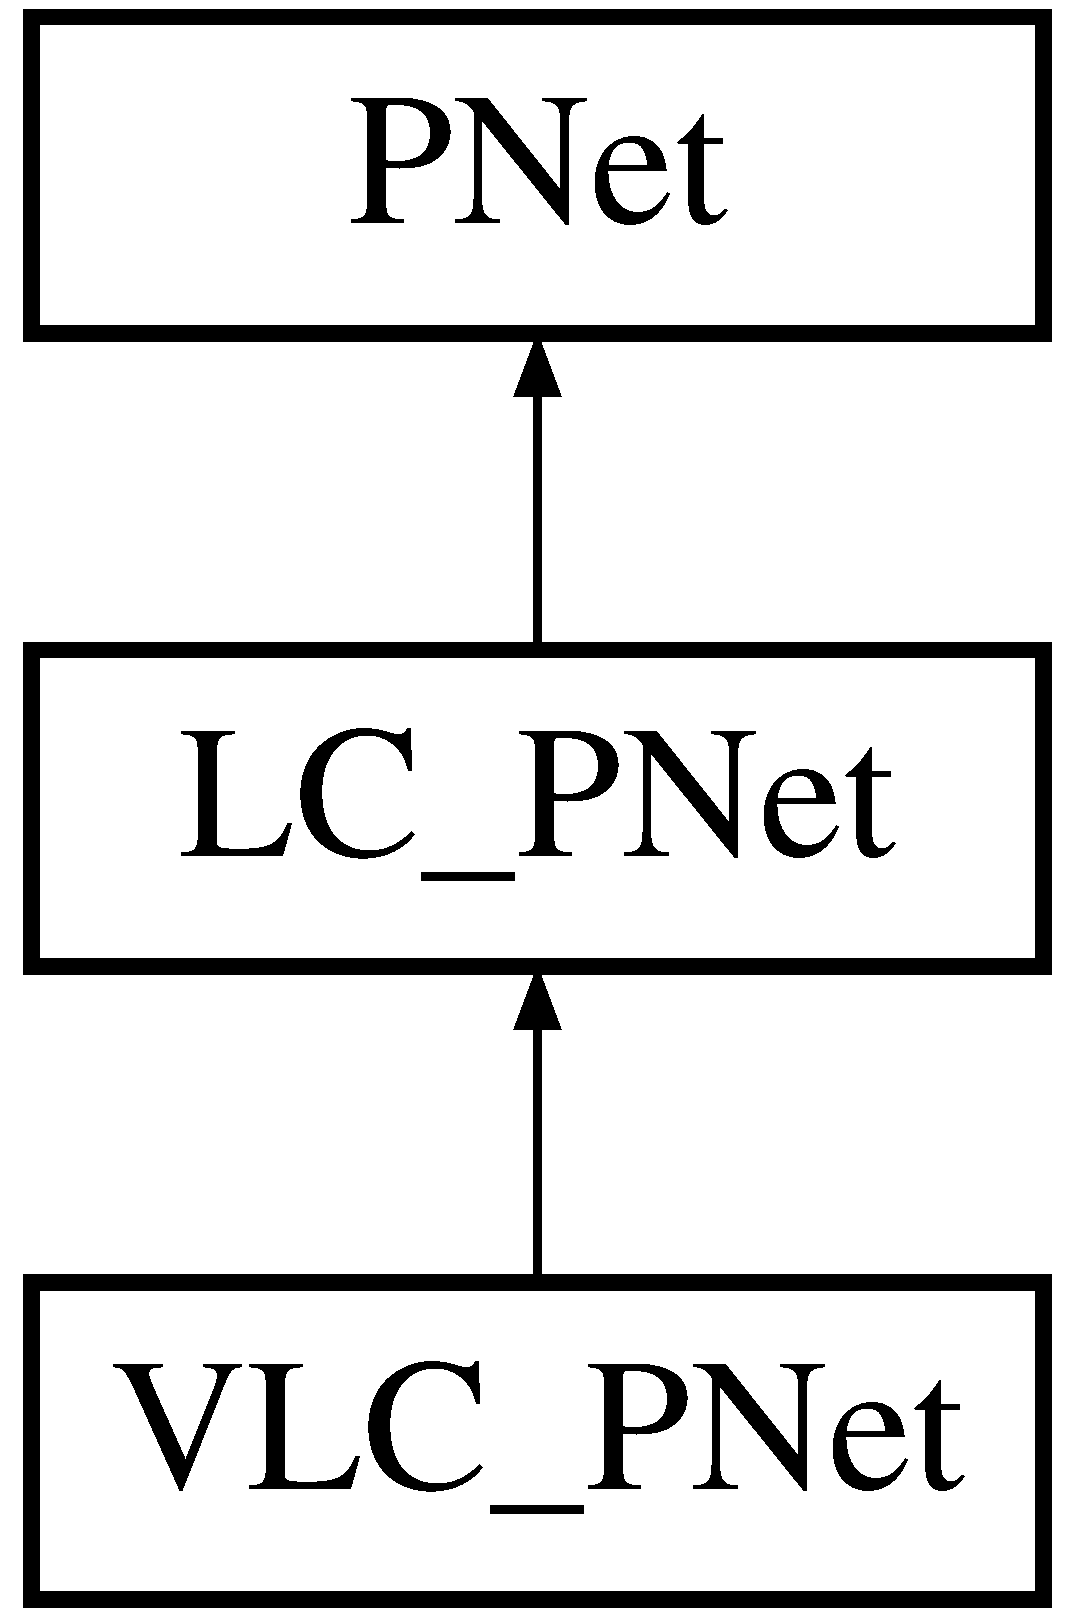
\includegraphics[height=3.000000cm]{class_l_c___p_net}
\end{center}
\end{figure}
\subsection*{Public Member Functions}
\begin{DoxyCompactItemize}
\item 
\hyperlink{class_l_c___p_net_a24f5b64eb7d135f812b05cfe747ddcc3}{L\+C\+\_\+\+P\+Net} (const int \&N, const int \&C, const int \&S)
\item 
\hypertarget{class_l_c___p_net_a699f289ae423aa2af17139502654ab81}{}void {\bfseries import\+\_\+connections} (const std\+::string \&filename)\label{class_l_c___p_net_a699f289ae423aa2af17139502654ab81}

\item 
\hypertarget{class_l_c___p_net_afedba98cfd4a57742b963bf1fefdebed}{}void {\bfseries print\+\_\+cm} ()\label{class_l_c___p_net_afedba98cfd4a57742b963bf1fefdebed}

\item 
\hypertarget{class_l_c___p_net_ac66589462b8882839a7a9849ce2025fa}{}void {\bfseries save\+\_\+states\+\_\+to\+\_\+file} (const std\+::string \&filename)\label{class_l_c___p_net_ac66589462b8882839a7a9849ce2025fa}

\item 
\hypertarget{class_l_c___p_net_a1a66a51c4b649d64812d8c7eb49bda56}{}void {\bfseries save\+\_\+connections\+\_\+to\+\_\+file} (const std\+::string \&filename)\label{class_l_c___p_net_a1a66a51c4b649d64812d8c7eb49bda56}

\item 
\hypertarget{class_l_c___p_net_afef840ecfc8b5b3a9180ca3c8e7f821f}{}void {\bfseries save\+\_\+\+J\+\_\+to\+\_\+file} (const std\+::string \&filename)\label{class_l_c___p_net_afef840ecfc8b5b3a9180ca3c8e7f821f}

\item 
\hypertarget{class_l_c___p_net_ab9a618c5fc495ee199b420d0aa16758a}{}void {\bfseries connect\+\_\+units} (std\+::default\+\_\+random\+\_\+engine \&generator)\label{class_l_c___p_net_ab9a618c5fc495ee199b420d0aa16758a}

\item 
\hypertarget{class_l_c___p_net_a0308d587505adab982a9e4322b8ac9ba}{}void {\bfseries init\+\_\+network} (const \+\_\+\+\_\+fpv \&beta, const \+\_\+\+\_\+fpv \&U, const int \&p, const \+\_\+\+\_\+fpv \&a, const int $\ast$xi)\label{class_l_c___p_net_a0308d587505adab982a9e4322b8ac9ba}

\item 
\hypertarget{class_l_c___p_net_adadf57b63af5fc9238bb97df3b56381d}{}void {\bfseries start\+\_\+dynamics} (std\+::default\+\_\+random\+\_\+engine \&generator, const int \&p, const int \&tstatus, const int \&nupdates, const int $\ast$xi, const int \&pattern, const \+\_\+\+\_\+fpv \&a, const \+\_\+\+\_\+fpv \&U, const \+\_\+\+\_\+fpv \&w, const \+\_\+\+\_\+fpv \&g, const \+\_\+\+\_\+fpv \&tau, const \+\_\+\+\_\+fpv \&b1, const \+\_\+\+\_\+fpv \&b2, const \+\_\+\+\_\+fpv \&b3, const \+\_\+\+\_\+fpv \&beta, const int \&tx)\label{class_l_c___p_net_adadf57b63af5fc9238bb97df3b56381d}

\end{DoxyCompactItemize}
\subsection*{Protected Member Functions}
\begin{DoxyCompactItemize}
\item 
\hypertarget{class_l_c___p_net_a2925dc1c225646f4be3e466383812f14}{}void {\bfseries init\+\_\+states} (const \+\_\+\+\_\+fpv \&beta, const \+\_\+\+\_\+fpv \&U)\label{class_l_c___p_net_a2925dc1c225646f4be3e466383812f14}

\item 
\hypertarget{class_l_c___p_net_aef7091aa9525fb95c3f1df19f801b535}{}void {\bfseries update\+\_\+rule} (const int \&unit, const \+\_\+\+\_\+fpv buffer\mbox{[}$\,$\mbox{]}, const int \&pattern, const \+\_\+\+\_\+fpv \&U, const \+\_\+\+\_\+fpv \&w, const \+\_\+\+\_\+fpv \&g, const \+\_\+\+\_\+fpv \&tau, const \+\_\+\+\_\+fpv \&b1, const \+\_\+\+\_\+fpv \&b2, const \+\_\+\+\_\+fpv \&b3, const \+\_\+\+\_\+fpv \&beta, const int \&tx, const int \&t)\label{class_l_c___p_net_aef7091aa9525fb95c3f1df19f801b535}

\item 
\hypertarget{class_l_c___p_net_a184fb2c6b021c7a814954e9750347b1c}{}void {\bfseries evaluate\+\_\+m} (const int \&p, const \+\_\+\+\_\+fpv \&a, const int $\ast$xi, \+\_\+\+\_\+fpv m\mbox{[}$\,$\mbox{]})\label{class_l_c___p_net_a184fb2c6b021c7a814954e9750347b1c}

\item 
\hypertarget{class_l_c___p_net_a22278003507e1871152e4024002a7ff9}{}void {\bfseries init\+\_\+\+J} (const int \&p, const \+\_\+\+\_\+fpv \&a, const int $\ast$xi)\label{class_l_c___p_net_a22278003507e1871152e4024002a7ff9}

\end{DoxyCompactItemize}
\subsection*{Protected Attributes}
\begin{DoxyCompactItemize}
\item 
\hypertarget{class_l_c___p_net_ac6fbf61a77df3fefd1add38665e7b717}{}int {\bfseries C}\label{class_l_c___p_net_ac6fbf61a77df3fefd1add38665e7b717}

\item 
\hypertarget{class_l_c___p_net_ab6a71cf2a87d2a84ef26d63da7cb28c7}{}int {\bfseries S}\label{class_l_c___p_net_ab6a71cf2a87d2a84ef26d63da7cb28c7}

\item 
\hypertarget{class_l_c___p_net_a4d5e6bfeff710d069640abaabf92e9d8}{}int $\ast$ {\bfseries cm}\label{class_l_c___p_net_a4d5e6bfeff710d069640abaabf92e9d8}

\item 
\hypertarget{class_l_c___p_net_a07424445de5664c7840fa76867d01491}{}\+\_\+\+\_\+fpv $\ast$ {\bfseries J}\label{class_l_c___p_net_a07424445de5664c7840fa76867d01491}

\item 
\hypertarget{class_l_c___p_net_a4c085a26d4bc5cc9c048f5652bf7d3c7}{}\+\_\+\+\_\+fpv $\ast$ {\bfseries active\+\_\+states}\label{class_l_c___p_net_a4c085a26d4bc5cc9c048f5652bf7d3c7}

\item 
\hypertarget{class_l_c___p_net_aa286239886cffadfb0098b4af9391cfd}{}\+\_\+\+\_\+fpv $\ast$ {\bfseries inactive\+\_\+states}\label{class_l_c___p_net_aa286239886cffadfb0098b4af9391cfd}

\item 
\hypertarget{class_l_c___p_net_af1e4cb3b01d9eea8dc4ee932ac486f5f}{}int $\ast$ {\bfseries ucm}\label{class_l_c___p_net_af1e4cb3b01d9eea8dc4ee932ac486f5f}

\item 
\hypertarget{class_l_c___p_net_a232191ada434e427069b9d73a32c6c11}{}\+\_\+\+\_\+fpv $\ast$ {\bfseries active\+\_\+r}\label{class_l_c___p_net_a232191ada434e427069b9d73a32c6c11}

\item 
\hypertarget{class_l_c___p_net_a4eefb8f8377ce107099d63bbc3b129bf}{}\+\_\+\+\_\+fpv $\ast$ {\bfseries inactive\+\_\+r}\label{class_l_c___p_net_a4eefb8f8377ce107099d63bbc3b129bf}

\item 
\hypertarget{class_l_c___p_net_a0f89876853795e0366d6f771295ec785}{}\+\_\+\+\_\+fpv $\ast$ {\bfseries h}\label{class_l_c___p_net_a0f89876853795e0366d6f771295ec785}

\item 
\hypertarget{class_l_c___p_net_ab4352d5dd32171b45a3471be0de07a77}{}\+\_\+\+\_\+fpv $\ast$ {\bfseries theta}\label{class_l_c___p_net_ab4352d5dd32171b45a3471be0de07a77}

\item 
\hypertarget{class_l_c___p_net_ade19ecf3ac391db683a740bde9fde66b}{}int $\ast$ {\bfseries xi}\label{class_l_c___p_net_ade19ecf3ac391db683a740bde9fde66b}

\end{DoxyCompactItemize}
\subsection*{Additional Inherited Members}


\subsection{Constructor \& Destructor Documentation}
\hypertarget{class_l_c___p_net_a24f5b64eb7d135f812b05cfe747ddcc3}{}\index{L\+C\+\_\+\+P\+Net@{L\+C\+\_\+\+P\+Net}!L\+C\+\_\+\+P\+Net@{L\+C\+\_\+\+P\+Net}}
\index{L\+C\+\_\+\+P\+Net@{L\+C\+\_\+\+P\+Net}!L\+C\+\_\+\+P\+Net@{L\+C\+\_\+\+P\+Net}}
\subsubsection[{L\+C\+\_\+\+P\+Net(const int \&\+N, const int \&\+C, const int \&\+S)}]{\setlength{\rightskip}{0pt plus 5cm}L\+C\+\_\+\+P\+Net\+::\+L\+C\+\_\+\+P\+Net (
\begin{DoxyParamCaption}
\item[{const int \&}]{N, }
\item[{const int \&}]{C, }
\item[{const int \&}]{S}
\end{DoxyParamCaption}
)}\label{class_l_c___p_net_a24f5b64eb7d135f812b05cfe747ddcc3}
\char`\"{}£\char`\"{} 

The documentation for this class was generated from the following files\+:\begin{DoxyCompactItemize}
\item 
/home/deathquasar/\+Projects/\+M\+H\+P\+C/\+Thesis/\+Code/\+Potts\+\_\+code/include/lc\+\_\+pnet.\+h\item 
/home/deathquasar/\+Projects/\+M\+H\+P\+C/\+Thesis/\+Code/\+Potts\+\_\+code/lib/lc\+\_\+pnet.\+cpp\end{DoxyCompactItemize}

\hypertarget{structparameters}{}\section{parameters Struct Reference}
\label{structparameters}\index{parameters@{parameters}}
\subsection*{Public Attributes}
\begin{DoxyCompactItemize}
\item 
int {\bfseries N}\hypertarget{structparameters_a0b2132a2da84d48e4575f6d9e8e899ee}{}\label{structparameters_a0b2132a2da84d48e4575f6d9e8e899ee}

\item 
int {\bfseries C}\hypertarget{structparameters_a2143fd1bb0b1132240b2ac1f48797837}{}\label{structparameters_a2143fd1bb0b1132240b2ac1f48797837}

\item 
int {\bfseries p}\hypertarget{structparameters_a83fbd6f42d209aab6d3aa8360835cb55}{}\label{structparameters_a83fbd6f42d209aab6d3aa8360835cb55}

\item 
int {\bfseries S}\hypertarget{structparameters_a491bc36fe07cd5249f7d54fd82f7cb63}{}\label{structparameters_a491bc36fe07cd5249f7d54fd82f7cb63}

\item 
int {\bfseries nupdates}\hypertarget{structparameters_adaa744c06c33db9f1116ddd62bf97303}{}\label{structparameters_adaa744c06c33db9f1116ddd62bf97303}

\item 
int {\bfseries Num\+Set}\hypertarget{structparameters_a7308970e43d375353d1fccc1e581a8f4}{}\label{structparameters_a7308970e43d375353d1fccc1e581a8f4}

\item 
int {\bfseries N\+\_\+fact}\hypertarget{structparameters_a3fd36b05da1943711146096ac4528c92}{}\label{structparameters_a3fd36b05da1943711146096ac4528c92}

\item 
int {\bfseries Num\+\_\+fact}\hypertarget{structparameters_a9d567a9e2b598ee9fbe8ac4ecd611bb4}{}\label{structparameters_a9d567a9e2b598ee9fbe8ac4ecd611bb4}

\item 
int {\bfseries tstatus}\hypertarget{structparameters_ab1a47a209b6cbeea981c2001aa48a603}{}\label{structparameters_ab1a47a209b6cbeea981c2001aa48a603}

\item 
\+\_\+\+\_\+fpv {\bfseries a}\hypertarget{structparameters_a855416f306051d9fafd42310c4c39e79}{}\label{structparameters_a855416f306051d9fafd42310c4c39e79}

\item 
\+\_\+\+\_\+fpv {\bfseries U}\hypertarget{structparameters_afe57c1c9613decd31b31cbe63744ca3a}{}\label{structparameters_afe57c1c9613decd31b31cbe63744ca3a}

\item 
\+\_\+\+\_\+fpv {\bfseries b1}\hypertarget{structparameters_a98a51cfec1fecb74da95181555bbacba}{}\label{structparameters_a98a51cfec1fecb74da95181555bbacba}

\item 
\+\_\+\+\_\+fpv {\bfseries b2}\hypertarget{structparameters_a80d5e1baec765e78bbb55eb4623344a3}{}\label{structparameters_a80d5e1baec765e78bbb55eb4623344a3}

\item 
\+\_\+\+\_\+fpv {\bfseries b3}\hypertarget{structparameters_ab90f8477078e4e234b38c0a17c537d6d}{}\label{structparameters_ab90f8477078e4e234b38c0a17c537d6d}

\item 
\+\_\+\+\_\+fpv {\bfseries beta}\hypertarget{structparameters_a18029b953bec42c937a931ecb083cfa2}{}\label{structparameters_a18029b953bec42c937a931ecb083cfa2}

\item 
\+\_\+\+\_\+fpv {\bfseries w}\hypertarget{structparameters_ab95743b50344ac26c8b78bdebc1c37d8}{}\label{structparameters_ab95743b50344ac26c8b78bdebc1c37d8}

\item 
\+\_\+\+\_\+fpv {\bfseries g}\hypertarget{structparameters_aec758045deddba9c9c7cb20fc7998fdd}{}\label{structparameters_aec758045deddba9c9c7cb20fc7998fdd}

\item 
\+\_\+\+\_\+fpv {\bfseries tau}\hypertarget{structparameters_a665737e3c32140c9dd8e023723eb45ac}{}\label{structparameters_a665737e3c32140c9dd8e023723eb45ac}

\item 
\+\_\+\+\_\+fpv {\bfseries a\+\_\+fact}\hypertarget{structparameters_a98eb1f46f30452fd05f1836db2cd483f}{}\label{structparameters_a98eb1f46f30452fd05f1836db2cd483f}

\item 
\+\_\+\+\_\+fpv {\bfseries eps}\hypertarget{structparameters_a612546fcd2f7f8c78055fa5be1a27dcd}{}\label{structparameters_a612546fcd2f7f8c78055fa5be1a27dcd}

\item 
\+\_\+\+\_\+fpv {\bfseries a\+\_\+pf}\hypertarget{structparameters_a4f824daf21865bb4be9134614cb0df38}{}\label{structparameters_a4f824daf21865bb4be9134614cb0df38}

\item 
\+\_\+\+\_\+fpv {\bfseries fact\+\_\+eigen\+\_\+slope}\hypertarget{structparameters_af7ed1eca879710da4d7521e6b14a5da2}{}\label{structparameters_af7ed1eca879710da4d7521e6b14a5da2}

\end{DoxyCompactItemize}


The documentation for this struct was generated from the following file\+:\begin{DoxyCompactItemize}
\item 
/home/deathquasar/\+Projects/\+M\+H\+P\+C/\+Thesis/\+Code/\+Potts\+\_\+code/include/parameters\+\_\+struct.\+h\end{DoxyCompactItemize}

\hypertarget{class_pattern_gen}{}\section{Pattern\+Gen Class Reference}
\label{class_pattern_gen}\index{Pattern\+Gen@{Pattern\+Gen}}
\subsection*{Public Member Functions}
\begin{DoxyCompactItemize}
\item 
\hypertarget{class_pattern_gen_ae347681b782de3d3b415f5e0212c687c}{}{\bfseries Pattern\+Gen} (const int N, const int p, const int S, const \+\_\+\+\_\+fpv a, const \+\_\+\+\_\+fpv beta, const int N\+\_\+fact, const int Num\+\_\+fact, const \+\_\+\+\_\+fpv a\+\_\+fact, const \+\_\+\+\_\+fpv eps, const \+\_\+\+\_\+fpv a\+\_\+pf, const \+\_\+\+\_\+fpv fact\+\_\+eigen\+\_\+slope)\label{class_pattern_gen_ae347681b782de3d3b415f5e0212c687c}

\item 
\hypertarget{class_pattern_gen_a1e77dc569b771ee5185f51c7ca900e1a}{}void {\bfseries generate} ()\label{class_pattern_gen_a1e77dc569b771ee5185f51c7ca900e1a}

\item 
\hypertarget{class_pattern_gen_ace5ff5d0cb3ccc4b8b4941a22096dbc2}{}void {\bfseries eval\+\_\+stats} ()\label{class_pattern_gen_ace5ff5d0cb3ccc4b8b4941a22096dbc2}

\item 
\hypertarget{class_pattern_gen_ae33872117e255a8db86ea50d1a9cb413}{}void {\bfseries save\+\_\+pattern\+\_\+to\+\_\+file} (const std\+::string filename)\label{class_pattern_gen_ae33872117e255a8db86ea50d1a9cb413}

\item 
\hypertarget{class_pattern_gen_a4c3e875c5a117b4fd3de9a83bc396df8}{}int $\ast$ {\bfseries get\+\_\+patt} ()\label{class_pattern_gen_a4c3e875c5a117b4fd3de9a83bc396df8}

\item 
\hypertarget{class_pattern_gen_aaceb7c87b9efea67ba77ca78e2352bae}{}int $\ast$ {\bfseries get\+\_\+patt} (const int n)\label{class_pattern_gen_aaceb7c87b9efea67ba77ca78e2352bae}

\end{DoxyCompactItemize}
\subsection*{Friends}
\begin{DoxyCompactItemize}
\item 
\hypertarget{class_pattern_gen_af18c1bfc19f67a8a280667eb030fb0d2}{}class {\bfseries P\+Network}\label{class_pattern_gen_af18c1bfc19f67a8a280667eb030fb0d2}

\end{DoxyCompactItemize}


The documentation for this class was generated from the following files\+:\begin{DoxyCompactItemize}
\item 
/home/deathquasar/\+Projects/\+M\+H\+P\+C/\+Thesis/\+Code/\+Potts\+\_\+code/include/pattern\+\_\+gen.\+h\item 
/home/deathquasar/\+Projects/\+M\+H\+P\+C/\+Thesis/\+Code/\+Potts\+\_\+code/lib/pattern\+\_\+gen.\+cpp\end{DoxyCompactItemize}

\hypertarget{class_p_net}{}\section{P\+Net Class Reference}
\label{class_p_net}\index{P\+Net@{P\+Net}}
Inheritance diagram for P\+Net\+:\begin{figure}[H]
\begin{center}
\leavevmode
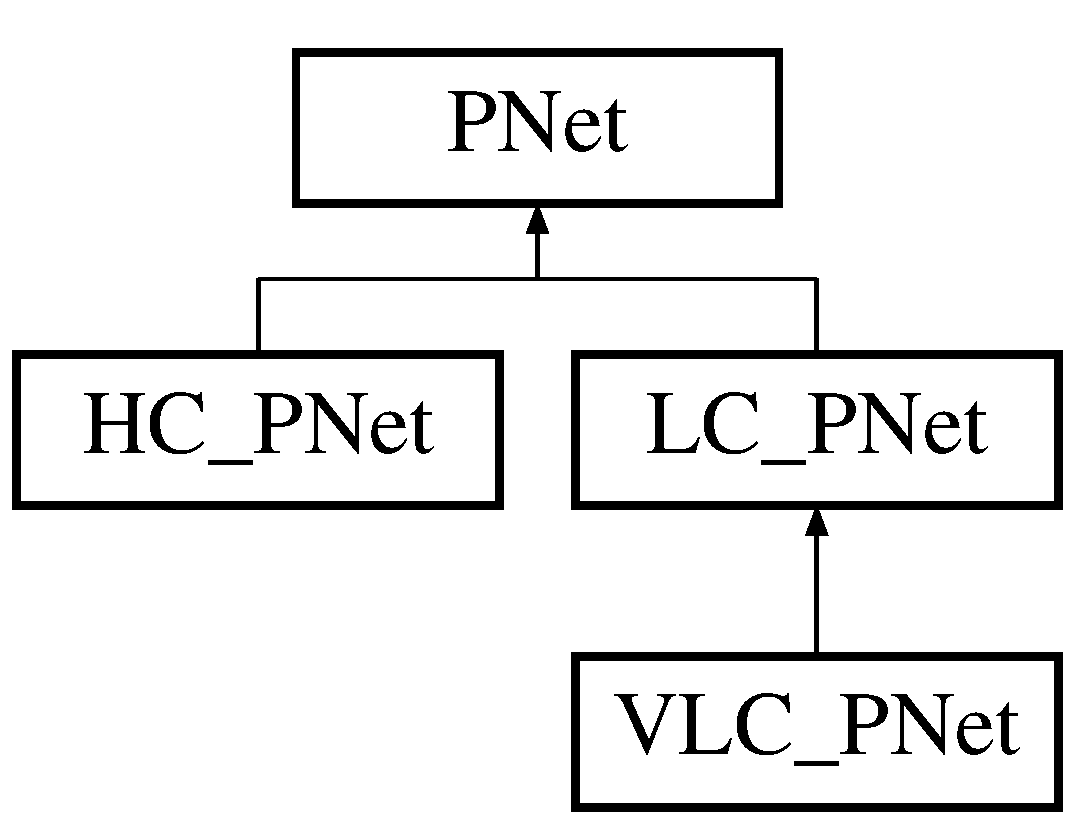
\includegraphics[height=3.000000cm]{class_p_net}
\end{center}
\end{figure}
\subsection*{Public Member Functions}
\begin{DoxyCompactItemize}
\item 
\hypertarget{class_p_net_ae7bb66e9b6e3cc8bebf69f0acc467978}{}{\bfseries P\+Net} (const int \&N)\label{class_p_net_ae7bb66e9b6e3cc8bebf69f0acc467978}

\item 
\hypertarget{class_p_net_af8319c3b3ec476d5008df5fe45c3544d}{}void {\bfseries print\+\_\+ksequence} ()\label{class_p_net_af8319c3b3ec476d5008df5fe45c3544d}

\item 
\hypertarget{class_p_net_a0f0c008ac7f00564bfdedfd3febd3602}{}virtual void {\bfseries print\+\_\+cm} ()=0\label{class_p_net_a0f0c008ac7f00564bfdedfd3febd3602}

\item 
\hypertarget{class_p_net_a2cac2b992ff0b0520f5dbb1a029676b1}{}virtual void {\bfseries save\+\_\+states\+\_\+to\+\_\+file} (const std\+::string \&filename)=0\label{class_p_net_a2cac2b992ff0b0520f5dbb1a029676b1}

\item 
\hypertarget{class_p_net_aad8dbda7540a1ed7d3fa142583770c0d}{}virtual void {\bfseries save\+\_\+connections\+\_\+to\+\_\+file} (const std\+::string \&filename)=0\label{class_p_net_aad8dbda7540a1ed7d3fa142583770c0d}

\item 
\hypertarget{class_p_net_a98feeb763aa03d366e6bf5b05c240f25}{}virtual void {\bfseries save\+\_\+\+J\+\_\+to\+\_\+file} (const std\+::string \&filename)=0\label{class_p_net_a98feeb763aa03d366e6bf5b05c240f25}

\item 
\hypertarget{class_p_net_a63efd6e2d7c5a38e0a6ae77af655a405}{}virtual void {\bfseries init\+\_\+network} (const \+\_\+\+\_\+fpv \&beta, const \+\_\+\+\_\+fpv \&U, const int \&p, const \+\_\+\+\_\+fpv \&a, const int $\ast$xi)=0\label{class_p_net_a63efd6e2d7c5a38e0a6ae77af655a405}

\item 
\hypertarget{class_p_net_afb427ff3050f26969782aec6bc76a5a7}{}virtual void {\bfseries start\+\_\+dynamics} (std\+::default\+\_\+random\+\_\+engine \&generator, const int \&p, const int \&tstatus, const int \&nupdates, const int $\ast$xi, const int \&pattern, const \+\_\+\+\_\+fpv \&a, const \+\_\+\+\_\+fpv \&U, const \+\_\+\+\_\+fpv \&w, const \+\_\+\+\_\+fpv \&g, const \+\_\+\+\_\+fpv \&tau, const \+\_\+\+\_\+fpv \&b1, const \+\_\+\+\_\+fpv \&b2, const \+\_\+\+\_\+fpv \&b3, const \+\_\+\+\_\+fpv \&beta, const int \&tx)=0\label{class_p_net_afb427ff3050f26969782aec6bc76a5a7}

\end{DoxyCompactItemize}
\subsection*{Public Attributes}
\begin{DoxyCompactItemize}
\item 
\hypertarget{class_p_net_ac21a9a2f6de2fc6094bdfacc78142ffe}{}\+\_\+\+\_\+fpv {\bfseries latching\+\_\+length}\label{class_p_net_ac21a9a2f6de2fc6094bdfacc78142ffe}

\end{DoxyCompactItemize}
\subsection*{Protected Member Functions}
\begin{DoxyCompactItemize}
\item 
\hypertarget{class_p_net_a6d519b171b571fccbc1d263ff40822e3}{}virtual void {\bfseries evaluate\+\_\+m} (const int \&p, const \+\_\+\+\_\+fpv \&a, const int $\ast$xi, \+\_\+\+\_\+fpv m\mbox{[}$\,$\mbox{]})=0\label{class_p_net_a6d519b171b571fccbc1d263ff40822e3}

\item 
\hypertarget{class_p_net_aeef297a15dc839818cd560228c9b8236}{}virtual void {\bfseries init\+\_\+\+J} (const int \&p, const \+\_\+\+\_\+fpv \&a, const int $\ast$xi)=0\label{class_p_net_aeef297a15dc839818cd560228c9b8236}

\item 
\hypertarget{class_p_net_a3c22be54795d659f2ebab3725ad93946}{}void {\bfseries get\+\_\+status} (const int \&p, const int \&tx, const int \&t, const int $\ast$xi, const \+\_\+\+\_\+fpv \&a, int \&Mumaxold, int \&Mumax, int \&steps, bool \&stop)\label{class_p_net_a3c22be54795d659f2ebab3725ad93946}

\end{DoxyCompactItemize}
\subsection*{Protected Attributes}
\begin{DoxyCompactItemize}
\item 
\hypertarget{class_p_net_a165f64c0fb771ebbcb5851b27373cf30}{}int {\bfseries N}\label{class_p_net_a165f64c0fb771ebbcb5851b27373cf30}

\item 
\hypertarget{class_p_net_ab636bd102fd68c5801c1b907dba52e9d}{}std\+::vector$<$ int $>$ {\bfseries ksequence}\label{class_p_net_ab636bd102fd68c5801c1b907dba52e9d}

\end{DoxyCompactItemize}


The documentation for this class was generated from the following files\+:\begin{DoxyCompactItemize}
\item 
/home/deathquasar/\+Projects/\+M\+H\+P\+C/\+Thesis/\+Code/\+Potts\+\_\+code/lib/pnet.\+h\item 
/home/deathquasar/\+Projects/\+M\+H\+P\+C/\+Thesis/\+Code/\+Potts\+\_\+code/lib/pnet.\+cpp\end{DoxyCompactItemize}

\hypertarget{class_p_p_s}{}\section{P\+P\+S Class Reference}
\label{class_p_p_s}\index{P\+P\+S@{P\+P\+S}}
\subsection*{Static Public Member Functions}
\begin{DoxyCompactItemize}
\item 
\hypertarget{class_p_p_s_a25cae7ae5a03f02d8c44b2b9b163ebe6}{}static void {\bfseries start} ()\label{class_p_p_s_a25cae7ae5a03f02d8c44b2b9b163ebe6}

\end{DoxyCompactItemize}
\subsection*{Static Public Attributes}
\begin{DoxyCompactItemize}
\item 
\hypertarget{class_p_p_s_a4e924fe2bb5ac2451243e7adc4f943ef}{}static int {\bfseries pid}\label{class_p_p_s_a4e924fe2bb5ac2451243e7adc4f943ef}

\item 
\hypertarget{class_p_p_s_a499131be4386ab41cf334cf42170518e}{}static int {\bfseries comm\+\_\+size}\label{class_p_p_s_a499131be4386ab41cf334cf42170518e}

\item 
\hypertarget{class_p_p_s_a0e5dcc27effd740a9d7b8d65356b80c1}{}static std\+::vector$<$ \hyperlink{structparameters}{parameters} $>$ {\bfseries plist}\label{class_p_p_s_a0e5dcc27effd740a9d7b8d65356b80c1}

\end{DoxyCompactItemize}


The documentation for this class was generated from the following files\+:\begin{DoxyCompactItemize}
\item 
/home/deathquasar/\+Projects/\+M\+H\+P\+C/\+Thesis/\+Code/\+Potts\+\_\+code/include/parallel\+\_\+scheduler.\+h\item 
/home/deathquasar/\+Projects/\+M\+H\+P\+C/\+Thesis/\+Code/\+Potts\+\_\+code/lib/parallel\+\_\+scheduler.\+cpp\end{DoxyCompactItemize}

\hypertarget{class_random_sequence}{}\section{Random\+Sequence Class Reference}
\label{class_random_sequence}\index{Random\+Sequence@{Random\+Sequence}}
\subsection*{Public Member Functions}
\begin{DoxyCompactItemize}
\item 
\hypertarget{class_random_sequence_a010f044bbdf4e8be029ba7b936e5c7ae}{}{\bfseries Random\+Sequence} (const int N)\label{class_random_sequence_a010f044bbdf4e8be029ba7b936e5c7ae}

\item 
\hypertarget{class_random_sequence_ab6ca117e2c7d36bdcf4b808c4c9a4e3e}{}void {\bfseries shuffle} (std\+::default\+\_\+random\+\_\+engine \&generator)\label{class_random_sequence_ab6ca117e2c7d36bdcf4b808c4c9a4e3e}

\item 
\hypertarget{class_random_sequence_acf065adaf2b78987d23187bdd60081f0}{}void {\bfseries print} ()\label{class_random_sequence_acf065adaf2b78987d23187bdd60081f0}

\item 
\hypertarget{class_random_sequence_ac2483da3051c252afe0fcc0c703774c5}{}int $\ast$ {\bfseries begin} ()\label{class_random_sequence_ac2483da3051c252afe0fcc0c703774c5}

\item 
\hypertarget{class_random_sequence_a457062d456d29e8d8acbbe78f3a964db}{}int $\ast$ {\bfseries end} ()\label{class_random_sequence_a457062d456d29e8d8acbbe78f3a964db}

\item 
\hypertarget{class_random_sequence_a87bbb74fa6a1b4f7c4e1bd07f011c724}{}int {\bfseries get} (const int \&i)\label{class_random_sequence_a87bbb74fa6a1b4f7c4e1bd07f011c724}

\end{DoxyCompactItemize}


The documentation for this class was generated from the following files\+:\begin{DoxyCompactItemize}
\item 
/home/deathquasar/\+Projects/\+M\+H\+P\+C/\+Thesis/\+Code/\+Potts\+\_\+code/include/random\+\_\+seq.\+h\item 
/home/deathquasar/\+Projects/\+M\+H\+P\+C/\+Thesis/\+Code/\+Potts\+\_\+code/lib/random\+\_\+seq.\+cpp\end{DoxyCompactItemize}

\hypertarget{class_v_l_c___p_net}{}\section{V\+L\+C\+\_\+\+P\+Net Class Reference}
\label{class_v_l_c___p_net}\index{V\+L\+C\+\_\+\+P\+Net@{V\+L\+C\+\_\+\+P\+Net}}
Inheritance diagram for V\+L\+C\+\_\+\+P\+Net\+:\begin{figure}[H]
\begin{center}
\leavevmode
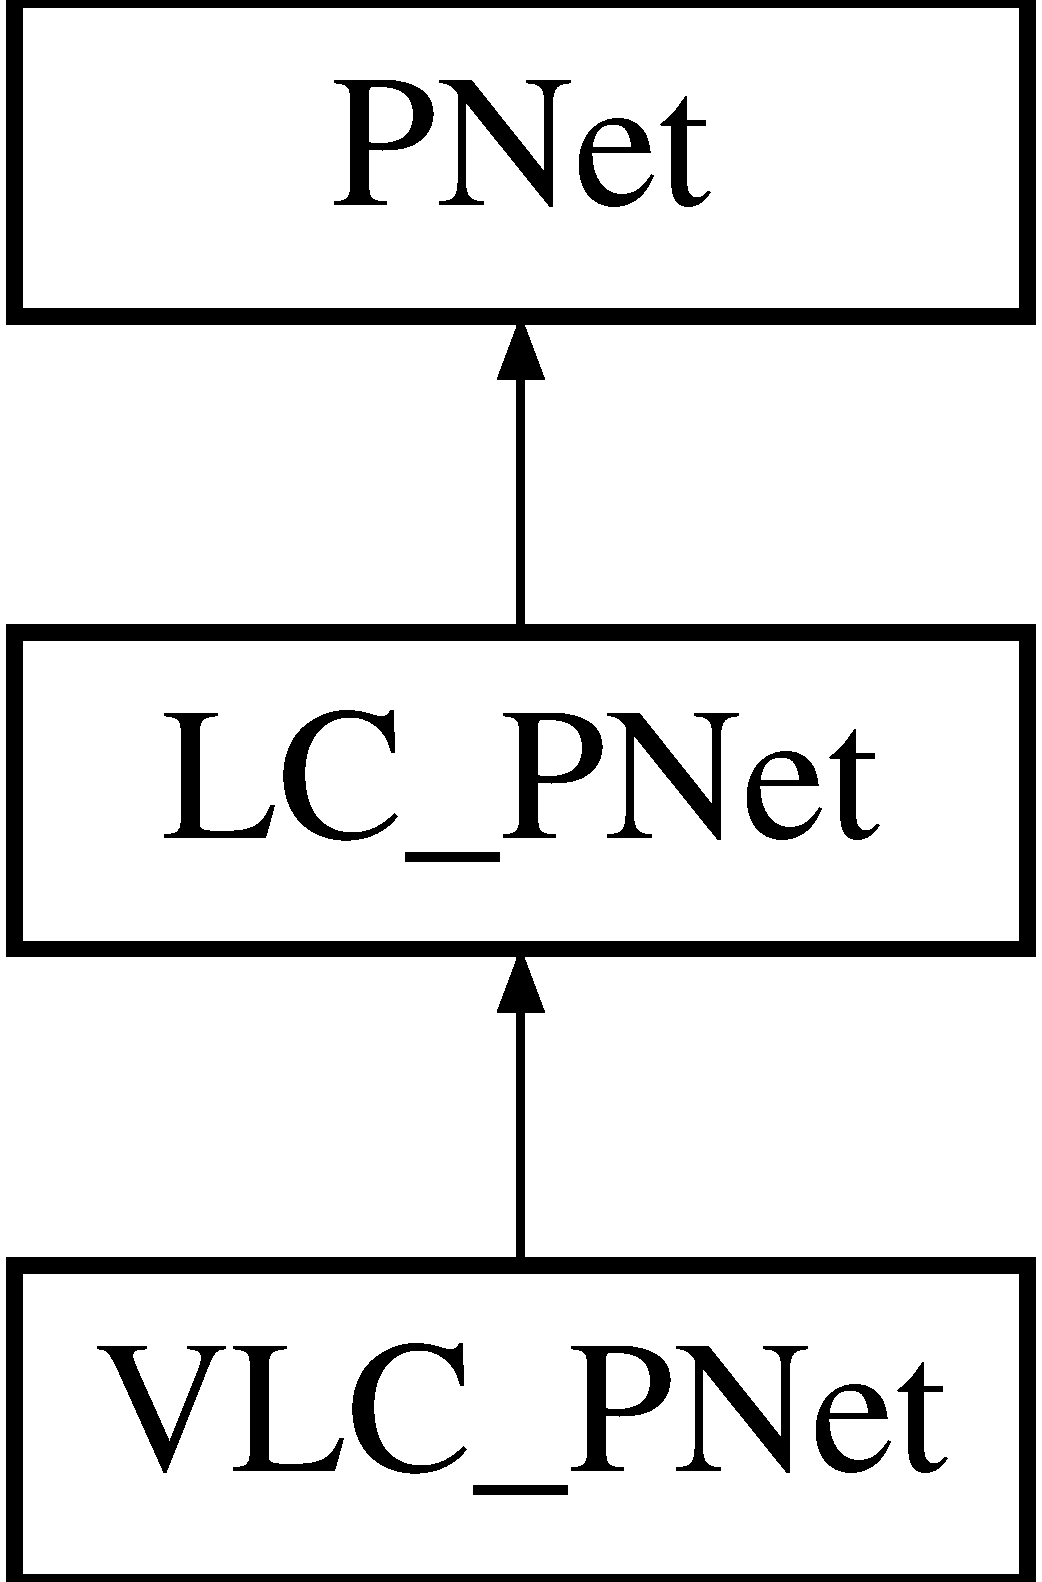
\includegraphics[height=3.000000cm]{class_v_l_c___p_net}
\end{center}
\end{figure}
\subsection*{Public Member Functions}
\begin{DoxyCompactItemize}
\item 
\hypertarget{class_v_l_c___p_net_a4c7e1b428ce72022e20ed2c7c05fc599}{}{\bfseries V\+L\+C\+\_\+\+P\+Net} (const int \&N, const int \&C, const int \&S)\label{class_v_l_c___p_net_a4c7e1b428ce72022e20ed2c7c05fc599}

\item 
\hypertarget{class_v_l_c___p_net_a8df456c85a7e6a0319a14c18f014a7d4}{}void {\bfseries start\+\_\+dynamics} (std\+::default\+\_\+random\+\_\+engine \&generator, const int \&p, const int \&tstatus, const int \&nupdates, const int $\ast$xi, const int \&pattern, const \+\_\+\+\_\+fpv \&a, const \+\_\+\+\_\+fpv \&U, const \+\_\+\+\_\+fpv \&w, const \+\_\+\+\_\+fpv \&g, const \+\_\+\+\_\+fpv \&tau, const \+\_\+\+\_\+fpv \&b1, const \+\_\+\+\_\+fpv \&b2, const \+\_\+\+\_\+fpv \&b3, const \+\_\+\+\_\+fpv \&beta, const int \&tx)\label{class_v_l_c___p_net_a8df456c85a7e6a0319a14c18f014a7d4}

\end{DoxyCompactItemize}
\subsection*{Additional Inherited Members}


The documentation for this class was generated from the following files\+:\begin{DoxyCompactItemize}
\item 
/home/deathquasar/\+Projects/\+M\+H\+P\+C/\+Thesis/\+Code/\+Potts\+\_\+code/include/vlc\+\_\+pnet.\+h\item 
/home/deathquasar/\+Projects/\+M\+H\+P\+C/\+Thesis/\+Code/\+Potts\+\_\+code/lib/vlc\+\_\+pnet.\+cpp\end{DoxyCompactItemize}

%--- End generated contents ---

% Index
\backmatter
\newpage
\phantomsection
\clearemptydoublepage
\addcontentsline{toc}{chapter}{Index}
\printindex

\end{document}
